%This is a experiment example of ZhengXiaoyang's experiment report template

\documentclass[UTF8]{ctexart}
 
\usepackage{amsmath}
\usepackage{cases}
\usepackage{cite}
\usepackage{ctex}
\usepackage{graphicx}
\usepackage[margin=1in]{geometry}
\geometry{a4paper}
\usepackage{fancyhdr}
\pagestyle{fancy}
\fancyhf{}

\graphicspath{{picture/}}


\title{利用双棱镜研究双光束干涉}
\graphicspath{{picture/}}


\title{利用双棱镜研究双光束干涉预习报告}
\author{郑晓旸}
\date{\today}
\pagenumbering{arabic}

\begin{document}
%这里是文件的开头
\fancyhead[L]{郑晓旸}
\fancyhead[C]{双棱镜干涉}
\fancyfoot[C]{\thepage}

\maketitle
\tableofcontents
\newpage

\section{实验目的}
    \begin{enumerate}
            \item 学习光路的调节方法;
            \item 学习用双棱镜干涉测量光波长的方法。
    \end{enumerate} 


\section{实验仪器}
\begin{enumerate}
    \item 光学导轨
    \item 钠灯
    \item 双棱镜
    \item 可调狭缝
    \item 凸透镜
    \item Cmos相机,型号MUS500C-G
\end{enumerate}

\section{实验原理}
\subsection{双光束干涉原理}
双光束干涉是指相干的两列波在空间相遇时,由于波的叠加而产生明暗相间的条纹。设两列相干光的复振幅分别为$\vec{E}_1$和$\vec{E}_2$,它们在空间某点P的振动方程为:\\
$$\vec{E}_1=\vec{A}_1e^{i(\omega t-\phi_1)}$$
$$\vec{E}_2=\vec{A}_2e^{i(\omega t-\phi_2)}$$
其中$\vec{A}_1$和$\vec{A}_2$分别为两列光在P点的振幅,$\phi_1$和$\phi_2$为相位。两列光在P点的合振幅为:
$$\vec{E}=\vec{E}_1+\vec{E}_2=\vec{A}_1e^{i(\omega t-\phi_1)}+\vec{A}_2e^{i(\omega t-\phi_2)}$$
光强与振幅的平方成正比,因此P点的光强为:
$$I=|\vec{E}|^2=|\vec{A}_1|^2+|\vec{A}_2|^2+2|\vec{A}_1||\vec{A}2|\cos\delta$$
其中$\delta=\phi_1-\phi_2$为两列光的相位差。可见光强与$\delta$有关,当$\delta$为偶数倍$\pi$时,光强取极大值$I_{max}=(|\vec{A}_1|+|\vec{A}2|)^2$;当$\delta$为奇数倍$\pi$时,光强取极小值$I_{min}=(|\vec{A}_1|-|\vec{A}_2|)^2$。这就是明暗相间的干涉条纹的形成原因。

\subsection{菲涅耳双棱镜干涉原理}
菲涅耳双棱镜是一种产生双光束干涉的装置。它由两块折射率相同的三棱镜组成,它们的一个面(底面)几乎重合,形成一个很小的二面角。当一束光垂直入射到双棱镜时,会被分成两束,分别经过上下两个棱镜,然后在棱镜后会聚成两个虚像光源$S_1$和$S_2$。

\begin{figure}[htbp]
    \centering
    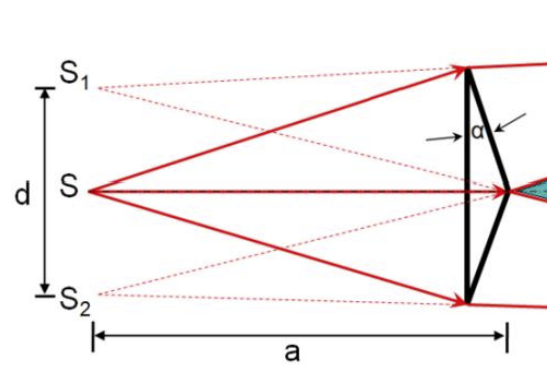
\includegraphics[width=0.6\textwidth]{prism}
    \caption{菲涅耳双棱镜分光示意图}
    \label{fig:fresnel_biprism}
\end{figure}

如图\ref{fig:fresnel_biprism}所示,设双棱镜的折射率为$n$,棱镜角为$\alpha$(一般很小,可认为$\sin\alpha\approx\alpha$),光源$S$到棱镜的距离为$d$。根据几何关系,可得两个虚像光源的间距为:
$$s=S_1S_2=2(n-1)d\alpha$$
在双棱镜后放一接收屏,到两个虚像光源的距离为$L$。在接收屏上任一点$P$,两束光程差为:
$$\delta=r_2-r_1\approx\frac{xs}{L}$$
其中$x$为$P$点到接收屏中心$O$的距离。代入双光束干涉的光强公式,可得:
$$I=4I_0\cos^2(\frac{\pi xs}{\lambda L})$$
其中$I_0$为单束光的光强。令$\Delta x=\frac{\lambda L}{s}$,则相邻亮纹间距为$\Delta x$,由此可得:
$$\lambda=\frac{\Delta xs}{L}$$
通过测量条纹间距$\Delta x$、虚像光源间距$s$以及接收屏到双棱镜的距离$L$,就可以计算出光的波长$\lambda$。

\subsection{虚像光源间距的测量}
为了测量虚像光源的间距$s$,可以在双棱镜后放一会聚透镜,分别在透镜的两个共轭面成像,测量两次像的大小,就可以计算出$s$。

\begin{figure}[!htbp]
    \centering
    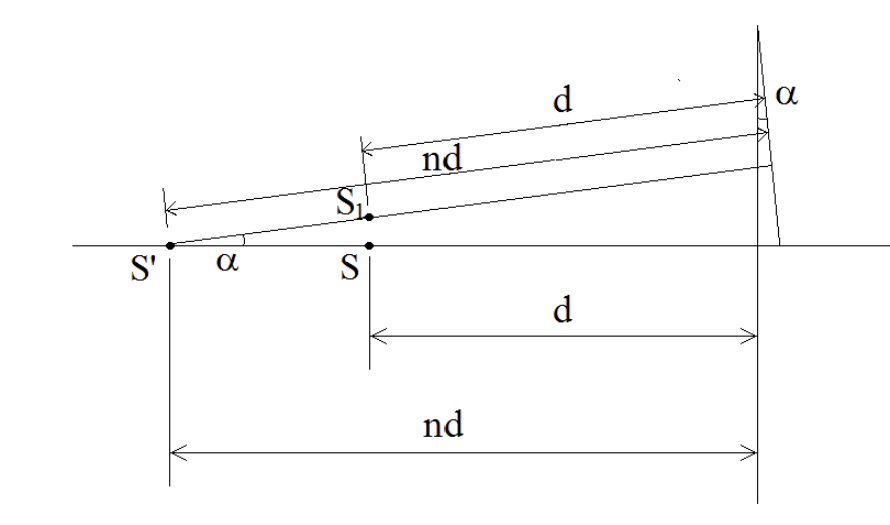
\includegraphics[width=0.8\textwidth]{sourced.png}
    \caption{虚像光源间距测量光路图}
    \label{fig:virtual_source_distance}
\end{figure}

如图\ref{fig:virtual_source_distance}所示,两个虚像光源$S_1$和$S_2$经过透镜成两次像$S_1'$和$S_2'$。当透镜与接收屏的距离为$L_1$时,物距为$L_2$,像距为$L_1$,放大率为$\beta_1=\frac{L_1}{L_2}$;当透镜与接收屏的距离为$L_2$时,物距为$L_1$,像距为$L_2$,放大率为$\beta_2=\frac{L_2}{L_1}$。两次成像的放大率互为倒数,即$\beta_1\beta_2=1$。
设第一次成像测得的像间距为$D_1$,第二次为$D_2$,则:
$$s=\frac{D_1}{\beta_1}=D_1\beta_2=\sqrt{D_1D_2}$$
这就是虚像光源间距$s$的计算公式。

以上就是该实验的主要原理,包括双光束干涉原理、菲涅耳双棱镜干涉原理以及虚像光源间距的测量方法。通过测量干涉条纹间距、虚像光源间距以及接收屏到双棱镜的距离,就可以计算出光的波长。



\section{实验方法}
本实验在光学导轨上进行,使用的主要器件包括钠灯、可调狭缝、菲涅耳双棱镜、会聚透镜和CMOS相机。实验装置如图\ref{fig:setup}所示。

\begin{figure}[htbp]
    \centering
    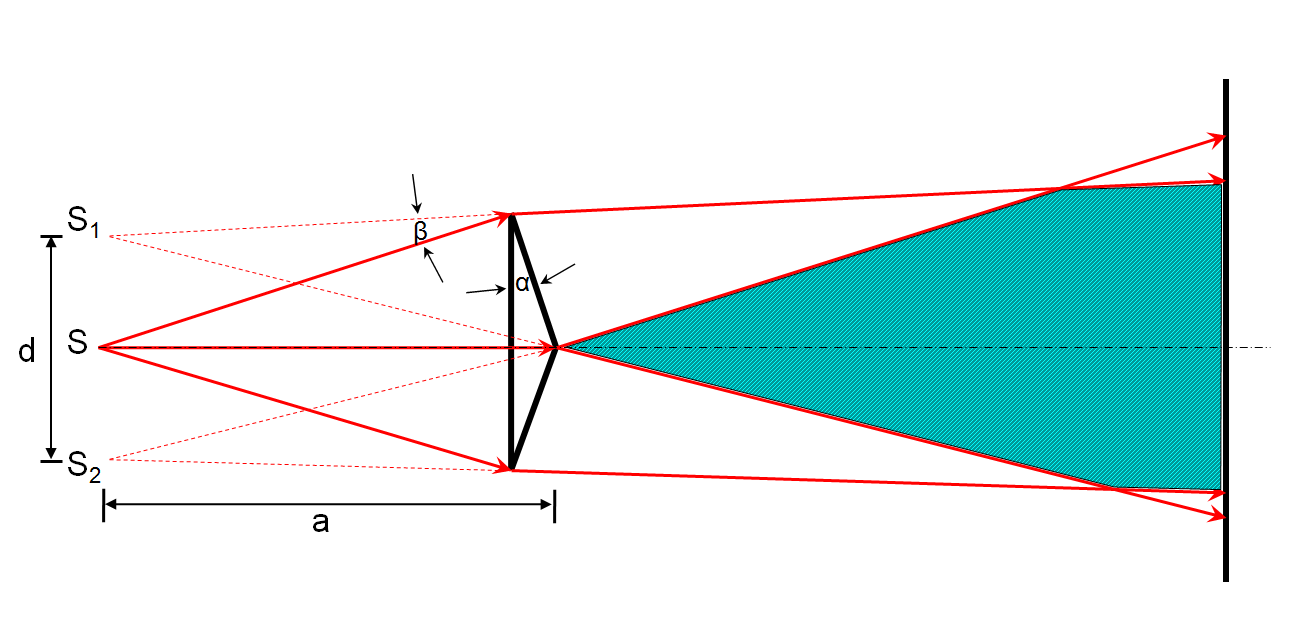
\includegraphics[width=0.8\textwidth]{ray.png}
    \caption{实验装置示意图}
    \label{fig:setup}
\end{figure}

具体实验步骤如下:

\begin{enumerate}
    \item 光路调节
    \begin{enumerate}
        \item 按照钠灯、狭缝、双棱镜、会聚透镜和相机的顺序在导轨上排列各个器件,大致调节各器件的高度,使其光轴在同一水平线上。
        \item 点亮钠灯,调节狭缝宽度至0.1mm左右。移动会聚透镜,使其在透镜两侧分别成一次狭缝的像,调节狭缝和透镜的位置,使成像清晰且像的大小不同。
        \item 在狭缝和透镜之间插入双棱镜,调节双棱镜的位置和角度,使通过双棱镜后狭缝像分裂成两条清晰的亮线。
        \item 移走会聚透镜,在双棱镜后放置相机,调节相机位置,使其能观察到清晰的干涉条纹。
    \end{enumerate}
    
    \item 波长测量
    \begin{enumerate}
        \item 测量干涉条纹间距$\Delta x$:用相机采集干涉条纹图像,选取多组清晰的条纹,测量其间距,取平均值作为$\Delta x$。
        \item 测量虚像光源间距$s$:在双棱镜后放置会聚透镜,移动透镜位置,使其成两次狭缝虚像的像,测量两次像间距$D_1$和$D_2$,根据公式$s=\sqrt{D_1D_2}$计算出$s$。
        \item 测量接收屏到双棱镜的距离$L$:直接用刻度尺测量相机CMOS面到双棱镜的距离。
        \item 计算波长$\lambda$:将测得的$\Delta x$、$s$和$L$代入公式$\lambda=\frac{\Delta xs}{L}$,计算出钠光波长$\lambda$。
    \end{enumerate}
    
    \item 数据处理与误差分析
    \begin{enumerate}
        \item 对多次测量的波长取平均值作为最终结果,计算波长的不确定度。
        \item 分析误差来源,主要包括$\Delta x$、$s$和$L$的测量误差。
    \end{enumerate}
\end{enumerate}

通过合理的实验操作和数据处理,可以较为精确地测量出钠黄光的波长,验证双光束干涉的基本规律。

\section{预习思考题}
\begin{enumerate}
    \item{\textbf{Q.1}} 假如将双棱镜旋转 180°,使顶角正对光源,虚光源的间距是否改变?\\ 
    \textbf{A.1}不改变。因为双棱镜的折射率和角度都没有改变,且物距不变,所以虚光源的间距不会改变。
    \item{\textbf{Q.2}}在用2 次成像法测量虚光源间距时,为了保证缩小像的间距不小于放大像间距的一半,
    狭缝与测微目镜的距离应满足什么条件?\\
    \textbf{A.2}为了保证缩小像的间距不小于放大像间距的一半,狭缝与测微目镜的距离应满足:
    $$L\leq 4f$$
    其中$L$为狭缝与测微目镜的距离,$f$为会聚透镜的焦距。\\
    当$L=4f$时,放大像与缩小像的距离相等,都等于$2f$。当$L<4f$时,缩小像的间距大于放大像间距的一半。

\end{enumerate}

\end{document}
